\section{Concepts}

\bitmz
  \itm 컴퓨터 시스템을 구성하는 네 가지 요소: \begin{figure}[h]\centering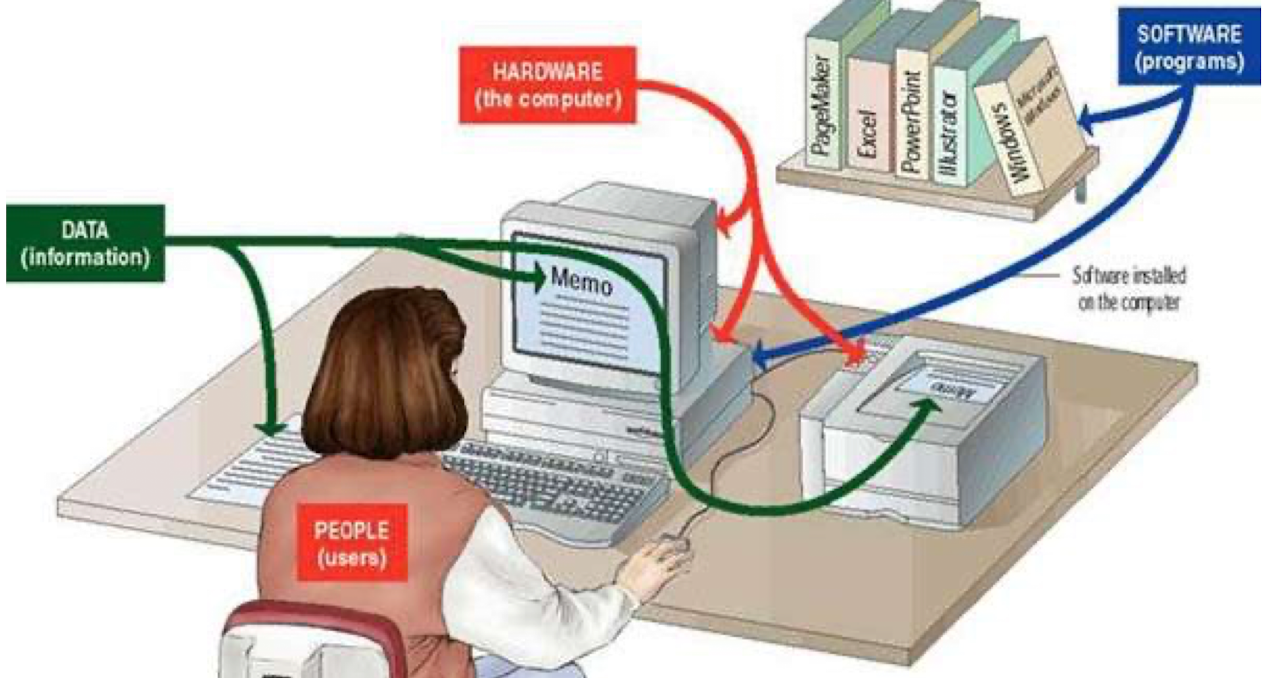
\includegraphics[width=7cm]{computer-system.png}\end{figure}
  \itm 컴퓨터 하드웨어의 블록 다이어그램: CPU는 메모리를 통해서만 데이터를 받을 수 있다. 입출력을 받는 메모리의 세 부분이 버퍼. 장치에서 온 데이터를 임시 저장하는 공간. 입력장치에서 출력을 내려면 메모리의 아웃풋 버퍼에 데이터를 전달해야 함. \begin{figure}[h]\centering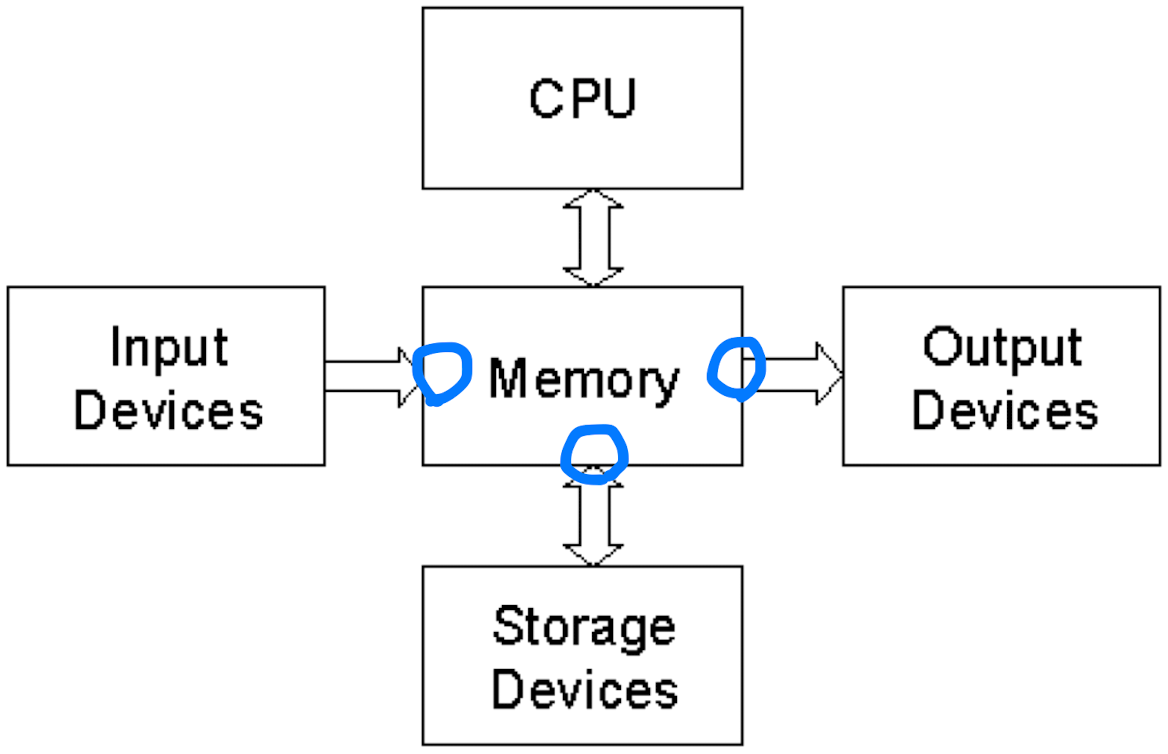
\includegraphics[width=7cm]{hardware-system.png}\end{figure}
  \itm 리눅스 소프트웨어: 실제로 모니터에 출력해주는 건 커널. \begin{figure}[h]\centering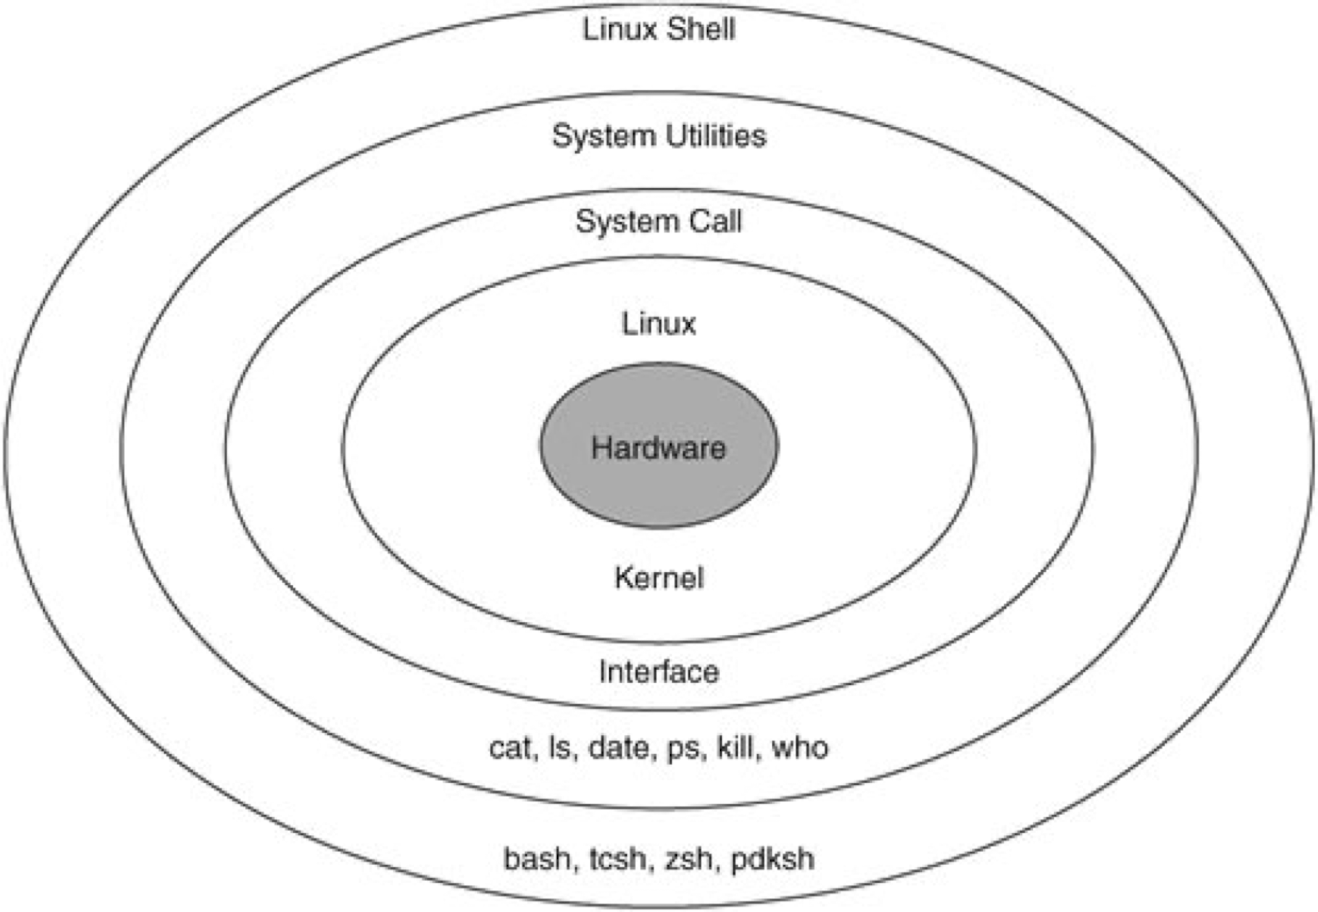
\includegraphics[width=7cm]{linux-software.png}\end{figure}
  \itm 프로세스의 3가지 상태:
  \bitmz
    \itm RUN(FG, BG): 명령을 백그라운드로 실행. e.g., \code{sleep 100 \&}
    \itm KILL: <Ctrl-c>
    \itm STOP: <Ctrl-z>
  \eitmz
  \itm EOF: <Ctrl-d>
  \itm 리눅스 파일 시스템은 트리 구조.
\eitmz

\section{Shell}

\bitmz
  \itm \code{!!} \rarr 직전 명령.
  \itm \code{\$?} \rarr 직전 명령의 리턴 값(exit status).
  \itm \code{\$!} \rarr 직전 프로세스의 아이디. e.g., \code{kill -9 \$!}
  \itm \code{!so} \rarr 가장 최근에 실행한 so로 시작하는 명령.
  \itm \code{a\%b} \rarr a에서 b를 제외한 문자열을 반환.

  \itm Redirection: 프로세스의 입출력 대상 파일을 변경.
  \bitmz
    \itm \code{>} stdout 방향 파일 지정 (덮어쓰기, clobbering). 덮어쓰기를 방지하려면 \code{shopt -o noclobber}.
    \bitmz
      \itm \code{ls x nf > file} \rarr stdout이 file에 쓰여지고, nf가 없다는 에러는 stderr에 출력.
      \itm \code{ls x nf 2> /dev/null} \rarr stdout이 출력되고, nf가 없다는 에러는 무시.
      \itm \code{ls x nf \&> file} \rarr stdout과 stdin이 file에 쓰여짐. \code{ls x nf > file 2>\&1}과 동일.
      \itm \code{wc 0< infile 1> outfile} \rarr infile을 stdin에, outfile을 stdout에 연결.
      \itm \code{cat result > file 2>\&1} \rarr stdout은 file에, stderr을 stdout에 연결. 즉, stdout과 stderr 모두 file에 기록된다. \&를 붙이지 않으면 file descriptor가 아닌 파일명으로 인식한다. 이때 \code{> file}과 \code{2>\&1}의 순서가 바뀌면 안 된다.
      \itm redirection하면 파일이 우선 만들어진다. \code{ls file > file}하면 에러가 나지 않고 파일에 file이 기록됨.
    \eitmz
    \itm \code{>>} stdout 방향 파일 지정 (이어쓰기)
    \itm \code{<} 파일을 stdin으로 전달.
    \itm \code{<<} here document. e.g., \code{cat <<EOF}.
    \itm \code{<<<} here string. 문자열을 stdin으로 전달. 사실상 \code{< /tmp/file}과 같다.
    \bitmz
      \itm \code{cat <<< string} \rarr \code{string} (\code{<<<}는 문자열 끝에 newline을 붙인다.)
      \itm \code{3<<< hello <\&3 cat} \rarr \code{hello} (\code{<\&3}은 \code{0<\&3})
    \eitmz
  \eitmz

  \itm Pipe (\code{a | b}) a 명령의 stdout을 b 명령의 stdin으로 전달.
  \bitmz
    \itm Pipe는 항상 sub shell에서 실행된다.
    \itm \code{|\&} \rarr 백그라운드 실행한 것을 파이프로 전달. \code{ls file |\& wc -l}는 1.
  \eitmz

  \itm Execution: \code{bash}, \code{source}, \code{./file.sh}
  \bitmz
    \itm \code{bash file.sh} 새로운 bash에서 file.sh를 실행. child process에서 실행되므로 parent가 export한 변수에만 접근할 수 있음.
    \itm 새 shell을 만들지 않고 실행하려면 \code{source} 또는 \code{./file.sh}한다. 마찬가지로 child process에서 실행.
    \itm 파일에서 선언한 변수는 그 안에서만 유효. 그런데 \code{source}하면 바깥에도 영향을 미침.
  \eitmz

  \itm Expansion
  \bitmz
    \itm \code{echo "A=\$A"} \rarr \code{A=100}
    \itm \code{echo 'A=\$A'} \rarr \code{A=\$A} (no expansion)
    \itm \code{echo "ab\$Ade"} \rarr \code{ab}, Ade는 없는 변수이므로 \code{echo "ab\$\{A\}de"} 이렇게 해야 한다.
    \itm \code{echo `which cc`} \rarr \code{which cc} 명령이 실행됨.
    \itm \code{add `add 100 200` 300} \rarr \code{600}
    \itm \code{\{n..m..k\}} k 간격으로 n부터 m까지 출력.
    \bitmz
      \itm \code{echo \{a,b,c\}.js} \rarr \code{a.js b.js c.js}
      \itm \code{echo \{0..5\}} \rarr \code{1 2 3 4 5}
      \itm \code{echo \{0..10..3\}} \rarr \code{0 3 6 9}
      \itm \code{echo \{a..z\}} \rarr a부터 z
    \eitmz
    \itm \code{\$\{ \}} variable expansion
    \bitmz
      \itm \code{echo \$\{STR:(-3):3\}} \rarr STR의 마지막 세 번째 글자부터 세 글자.
      \itm \code{echo \$\{STR/from/to\}} \rarr STR의 from 문자열을 to로 변경.
      \itm \code{echo \$\{STR:-ALT\}} \rarr STR이 unset되어 있는 경우 ALT를 출력.
      \itm \code{echo \$\{STR:+ALT\}} \rarr STR이 set되어 있는 경우 ALT를 출력.
      \itm \code{echo \$\{PATH\#\#*.\}} \rarr PATH에서 .을 만날 때까지 문자를 제거. (extension)
      \itm \code{echo \$\{PATH\#\#*/\}} \rarr PATH에서 /를 만날 때까지 문자를 제거. (basename)
    \eitmz
    \itm \code{\$(( ))} numerical expansion: \code{echo $(( 100 + 200 ))$} \rarr 300
    \itm \code{\$( )} command substitution. 명령의 출력으로 치환한다. 백틱과 동일. e.g., \code{rm \$(cat file)}
  \eitmz


  \itm Function(\code{function fn() \{ ... ;\}}): 함수의 결과는 stdout으로 내야. return은 exit status. 인자는 \code{\$1, \$2, ...}으로 사용.

  \itm Condition
  \bitmz
    \itm \code{if [[ condition ]]; then command1; elif [[ condition2 ]]; then command2; else command3; fi}
    \itm \code{if [[ -z \$STR ]]; then echo "empty"; else echo "not empty"; fi}
    \itm \code{if [[ \$STR1 == \$STR2 ]]; then echo "eq"; else echo "neq"; fi}
    \itm \code{if (( \$NUM1 < \$NUM2 )); then echo "lt"; else echo "gt"; fi} (bracket을 쓰면 숫자가 아니라 문자 순서 비교.)
    \itm \code{if command1; then command2; else command3; fi} \rarr command1의 exit status에 따른 분기.
  \eitmz

  \itm Loop
  \bitmz
    \itm \code{for i in /etc/*; do echo \$i; done} \rarr \code{/etc} 아래 모든 파일명을 출력.
    \itm \code{for ((i = 0 ; i < 100 ; i++)); do echo \$i; done}
    \itm \code{cat file | while read i; do echo \$i; done}
    \itm \code{sum=0; for i in \{1..10\}; do sum=\$(( \$sum+\$i )); echo \$i ":" \$sum; done}
    \itm \code{for i in \{000..999\}; do touch file\_\$\{i\}.c; done} \rarr file\_000.c부터 file\_999.c 파일 생성. 사실 touch는 파일 생성이 아니라 수정날짜를 바꾸는 명령.
    \itm \code{for i in file\_*; do mv \$i \$\{i\%.c\}.rs; done} \rarr file\_로 시작하는 파일들을 순회하며 문자열 끝의 .c를 .rs로 바꾼다.
    \itm \code{sum=0; for i in \{7..999..7\}; do sum=\$(( \$sum+\$i )); done; echo \$sum} \rarr 999까지의 모든 7의 배수 출력.
  \eitmz

  \itm Variable
  \bitmz
    \itm \code{A=100} \rarr A를 set.
    \itm \code{unset -v A} \rarr A가 변수인 경우에만 unset.
    \itm \code{unset A} \rarr A가 함수인 경우에도 unset.
    \itm \code{compgen -A variable} \rarr 모든 변수명을 출력.
    \itm \code{export A} \rarr A를 child shell에서 사용할 수 있도록 export.
    \itm \code{read A} \rarr A에 사용자 입력을 저장.
    \bitmz
      \itm sub shell은 child shell과 달리 export되지 않은 변수에 접근할 수 있음. 하지만 sub shell에서 변경한 값이 외부에 반영되지는 않음. \code{A=100; (echo \$A; A=300; echo \$A); echo \$A} \rarr 100과 300이 출력된 뒤, 마지막에는 100이 출력.
    \eitmz
  \eitmz

  \itm Globbing(\code{*})
  \bitmz
    \itm \code{echo *} \rarr 모든 파일의 이름을 띄어쓰기 간격으로 출력.
    \itm \code{echo a*b} \rarr a로 시작해서 b로 끝나는 모든 파일("ab" 포함).
    \itm \code{echo a??b} \rarr a로 시작해서 임의의 2개 문자가 사이에 있고 b로 끝나는 모든 파일.
    \itm \code{echo [ab]*} \rarr a 또는 b로 시작하는 모든 파일.
    \itm \code{echo [ab][ab]*} \rarr aa, bb, ab, ba로 시작하는 모든 파일.
    \itm \code{echo *(aa|bb)} \rarr aa 또는 bb로 끝나는 모든 파일. 앞에 glob 없으면 파이프.
    \itm \code{echo ?(aa)} \rarr aa 0개 또는 1개 포함 모든 파일.
    \itm \code{echo +(aa|bb)} \rarr aa 또는 bb 1개 이상 포함 모든 파일. (aabbb는 안 됨)
    \itm \code{echo [!a]*} \rarr a로 시작하지 않는 모든 파일.
    \itm \code{[[:upper:]], [[:lower:]], [[:digit:]], [[:space:]], [[:alpha:]], [[:alnum:]]} \rarr 대문자, 소문자, 숫자 등.
    \itm \code{shopt -s globstar} \rarr \code{**}을 활성화한다. 서브 디렉토리까지 재귀적으로 탐색. e.g., \code{lib/**/*.c} \rarr lib 디렉토리 아래 모든 디렉토리에서 .c로 끝나는 파일을 찾는다.
    \itm \code{echo 'AAbb' | tr '[:lower:]' '[:upper:]'} \rarr \code{AABB}
  \eitmz

  \itm Group(\code{\{ ;\}}): 같은 컨텍스트로 묶는다.
  \bitmz
    \itm \code{time \{ sleep 1; sleep 2; echo done ;\}} \rarr 모든 명령의 실행 시간.
    \itm \code{\{ echo a ; echo b ;\} > file} \rarr file에 a와 b가 모두 저장됨.
  \eitmz

  \itm Sub shell(\code{()}): 새로운 컨텍스트.
  \bitmz
    \itm \code{(echo a; echo b) > file} \rarr file에 a와 b가 모두 저장됨.
  \eitmz
\eitmz

\section{Linux}

\bitmz
  \itm \code{ls} 파일 리스트.
  \bitmz
    \itm \code{ls file} \rarr 해당 파일이 있는지 여부. 있다면 stdout에 파일명을 출력, 없다면 stderr에 에러 메시지.
    \itm \code{ls -d dir} \rarr 디렉토리 내 파일 리스트가 아니라 dir을 출력. (해당 디렉토리가 있는지 여부) \code{ls -d}하면 . 출력.
    \itm \code{ls *.txt} \rarr \code{.txt}로 끝나는 모든 파일 출력.
    \itm \code{ls -i} \rarr INode를 함께 출력.
  \eitmz

  \itm \code{cat} 텍스트 파일인 경우 stdout에 출력, 아니면 최대한 텍스트 파일인 것처럼 stdout에 출력.

  \itm \code{fg}, \code{bg} 프로세스를 포그라운드/백그라운드로 전환한다. stdin을 기다리는 명령을 백그라운드에서 실행하면 STOP된다. 따라서 리디렉션으로 파일에서 입력을 받아야 한다.
  \itm \code{kill} 프로세스에 시그널을 보낸다.
  \bitmz
    \itm \code{kill -9 PID}
    \itm \code{kill \%JID} \rarr JID는 \code{jobs}했을 때 나오는 아이디.
  \eitmz

  \itm \code{chmod [ugoa][+-][rwx] files...} 파일의 권한을 변경한다.
  \bitmz
    \itm rwx(user)rwx(group)rwx(others) = all
    \itm r(4), w(2), x(1): e.g., \code{chmod 700 file}
    \itm \code{-R} 디렉토리 내 모든 파일에 재귀적으로 적용.
    \itm \code{/usr/bin/passwd}의 권한은 \code{-rws------}. \code{s}는 \code{setid}, 이 명령을 실행할 때 잠시 root 권한을 주는 것.
    \itm default permission은 \code{-rw-r--r--}. 이것을 umask라고 한다.
    \itm 퍼미션 오른쪽 숫자는 같은 INode를 공유하는 링크 개수. 디렉토리의 경우에는 포함된 파일 개수.
  \eitmz

  \itm \code{mv} 파일이나 디렉토리를 이동한다.
  \bitmz
    \itm \code{\$ mv dir1 dir2} \rarr dir1을 통째로 dir2 아래로 옮긴다.
  \eitmz

  \itm \code{ln} 링크를 만든다.
  \bitmz
    \itm \code{-s} 심볼릭 링크를 만든다. 심볼릭 링크의 퍼미션은 \code{l}로 시작.
    \itm 하드 링크는 같은 INode를 가리키는 파일을 만드는 것. 하드 링크로 만들어진 파일은 링크가 아니라 그냥 파일. 원본을 지워도 안 지워진다.
  \eitmz

  \itm \code{cp} 파일을 복사한다.
  \bitmz
    \itm \code{-a} 원본 파일의 속성(생성 날짜 등)을 보존.
  \eitmz

  \itm \code{gzip} 파일 압축: \code{gzip file.ext}, \code{gzip -d file.ext.gz}
  \itm \code{tar} 아카이브 파일 생성
  \bitmz
    \itm create a gzipped archive and write it to a file: \code{tar czf path/to/target.tar.gz path/to/file1 path/to/file2 ...}
    \itm Extract a (compressed) archive file into the current directory verbosely: \code{tar xvf path/to/source.tar[.gz|.bz2|.xz]}
  \eitmz
  \itm \code{passwd [user]} \rarr 비밀번호 변경
  \itm \code{who} \rarr 접속 유저 확인
  \itm \code{tty} \rarr 지금 사용하는 터미널 정보
  \itm \code{man [section] command} \rarr section 1: general commands, 2: system calls, ...
\eitmz
